\section{模板的使用说明}

将模板的压缩包下载,解压缩, 其中包括以下5项:
\begin{itemize}
  \item 文件夹Img, 用于存放课程论文需要的插图.
  \item  essay\_qfnu\_v1.tex, 这是tex源文件, 论文内容完全在该文件中输入.
  \item qfnu\_essay.sty, 这是格式文件, 包含论文的版面格式、数学公式、章节格式、定理环境等相关的宏包和命令, 不建议作者改动该文件.
  \item 说明.pdf, 本模板的说明文档.
  \item 校字【2008】95号文:曲阜师范大学本科课程论文(设计)管理办法(终稿).doc, 学校文件, 包含课程论文的Word模板.
\end{itemize}
在编译essay\_qfnu\_v1.tex文件时, 需要调用qfnu\_essay.sty格式文件和Img文件夹, 因此应当保证三者始终处于同一个目录(文件夹)下. 一般情况下, 编译两次才能生成完整的pdf文件.

注意, 本模板要在TexLive系统下编译.

课程论文的作者只需要在tex源文件相应位置输入以下内容:
\begin{itemize}
  \item 自定义命令. 有些命令比较长但是需要在论文中频繁用到, 有时候一些符号并不在系统中, 此时作者可以按照一定的格式自定义一些新的命令. 见图\ref{pic: redefine}.
        \begin{figure}
          \centering
          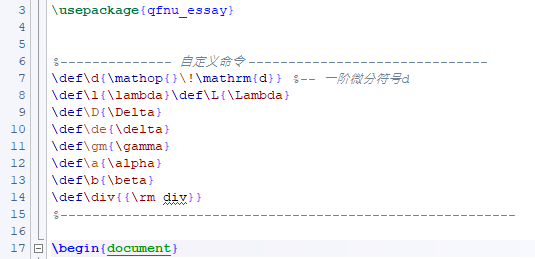
\includegraphics[width =4in]{Img/redefine.png}
          \caption{自定义命令}   %--- 插图标题 ---
          \label{pic: redefine} %--- 插图的引用标签---
        \end{figure}
  \item 基本信息: 论文标题, 专业, 学号, 作者姓名, 指导教师姓名, 依托课程. 见图\ref{pic: basic-info}.
        \begin{figure}
          \centering
          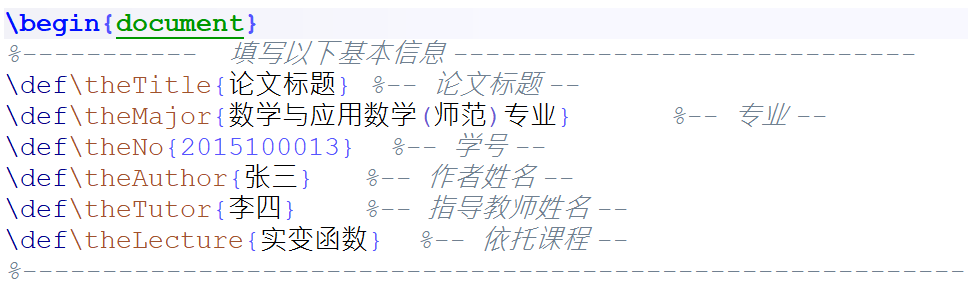
\includegraphics[width =4in]{Img/basic-info.png}
          \caption{基本信息}   %--- 插图标题 ---
          \label{pic: basic-info} %--- 插图的引用标签---
        \end{figure}
  \item 摘要和关键词.
  \item 正文内容.
  \item 参考文献. 列出的参考文献都要在正文中被引用, 否则不要出现.
\end{itemize}

